% !TEX program = xelatex

\documentclass[14pt]{beamer}

\usepackage{xeCJK}
\usepackage{fontspec,xunicode,xltxtra}
\setmonofont[Mapping={}]{Source Code Pro}
\setCJKmainfont[ItalicFont={AR PL UKai CN}, BoldFont={WenQuanYi Zen Hei}]{WenQuanYi Zen Hei}
\setCJKmonofont[BoldFont={WenQuanYi Zen Hei Mono}]{WenQuanYi Zen Hei Mono}
\setCJKsansfont[ItalicFont={AR PL UKai CN},BoldFont={WenQuanYi Zen Hei Mono}]{WenQuanYi Zen Hei}

\usepackage{mathtools}
\usepackage{graphics}
\usepackage{subfigure}

\usetheme{epyt}

\hypersetup{
  pdfpagemode={FullScreen},
}

\graphicspath{{figure/}{figures/}{logo/}{logos/}{graph/}{graphs}}

\title{社交网络中部分信息缺失下的社区发现}
\author{5090209296 李奇平}
\institute{指导教师:王灿、陈英}
\date{2013年6月17日}

\begin{document}

\begin{frame}[plain]\transboxout
\titlepage
\end{frame}

\begin{frame}\transboxin
\frametitle{主要内容}
\tableofcontents[hideallsubsections]
\end{frame}

\section{课题背景}

\begin{frame}{研究目的}
本文主要研究如何在信息缺失的社交网络中进行社区挖掘 \pause
\begin{itemize}[<+->]
\item 社交网络中的社区:联系比较密切的一组人
\item 信息缺失:无法获得社交网络的全部信息
\end{itemize}
\end{frame}

\begin{frame}[fragile]{本文思路}
\begin{enumerate}[<+->]
\item 利用局部信息网络的信息学习到一个距离度量;
\item 利用距离度量计算节点之间的距离;
\item 基于距离进行聚类;
\end{enumerate}
\end{frame}

%\begin{frame}[Emuerate]
%Epyt is a simple but nice theme for Beamer, with the following features: \pause
%\begin{itemize}[<+->]
%\item simple structure: with page numbers at footer, no head bar and side bar;
%\item simple templates: displaying theorems with traditional inline style;
%\item simple colors: using only three main colors - gray, yellow and white.
%\end{itemize}
%\end{frame}

\section{研究内容}

\begin{frame}{信息缺失网络}
尽管无法获取所有节点的信息,
但是可以得到少数几个局部信息网络,
局部信息网络中所有节点的信息是已知的。\pause

利用局部信息网络的信息,可以知道哪些节点是相似的,哪些节点是不相似的。
\end{frame}

\begin{frame}{距离度量学习——DCA}
\begin{itemize}[<+->]
    \item 距离度量:\[ d_o(X, Y) = \sqrt{(X - Y)(X - Y)}\] \[d_M(X, Y) = \sqrt{(X - Y)^\top M (X - Y)}\]
\item 目的:让已知的相似的节点距离更近
\item 最优化问题:\[ J(A) = \operatorname*{arg\,max}_A \frac {|A^\top \hat{C_b} A|} {|A^\top \hat{C_w} A|} \]
\item 结果:\[ M = A^\top A \]
\end{itemize}
\end{frame}

\begin{frame}{基于距离进行聚类——DSHRINK}
\begin{itemize}[<+->]
\item 层次聚类算法
\item 使用模块性准测终止算法的运行
\end{itemize}
\end{frame}

\begin{frame}{最近邻居与互紧邻}
\begin{itemize}
\item 最近邻居:\[
NN(v) = \{y | y = \operatorname*{arg\,min}_x d(u, x), x \in V \wedge x \neq v\}\]
\item
互近邻:
\[ u \xleftrightarrow{\gamma} v \text{当且仅当} \\
v \in NN(u) \wedge u \in NN(v) \wedge d(u, v) = \gamma \]
\end{itemize}
\end{frame}

\begin{frame}{当地社区}
$G = (V, E, A, M)$,
$C(v) = (V^\prime, E^\prime, A^\prime, M, \gamma)$是一个当地社区:

\[ v \in V^\prime \] \\
\[ \forall u \in V^\prime, \exists v \in V^\prime \wedge u \xleftrightarrow{\gamma} v \] \\
\[ \{u | u \in V^\prime \wedge u \xleftrightarrow{\gamma} v \wedge v \notin V^\prime \} = \emptyset \]
\end{frame}

\begin{frame}{模块性准则}

\[
Q_d = \sum_{i=1}^k [ \frac{D_i^I}{D^T} - (\frac{D_i^C}{D^T})^2]
\]

$Q_d$取值范围是[-1,0], $Q_d$越小,聚类的质量越好。

\end{frame}

\section{实验}

\begin{frame}{实验概述}
实验分为一下几个步骤:
\begin{itemize}
\item 选取数据集
\item 生成局部信息网络
\item 距离度量学习
\item 基于距离进行聚类
\end{itemize}

\begin{table}[!hpb]
\centering
\caption{实验采用数据集}
    \begin{tabular}{rrrrr} \toprule
    数据集 & 节点数 & 边数  & 属性数 & 类个数\\ \midrule
    Blogcatalog-a & 5118 & 22863 & 50 & 6 \\
    Blogcatalog-b & 5118 & 25761  & 50 & 6 \\ \bottomrule
    \end{tabular}
\end{table}
\end{frame}

\begin{frame}{评判标准}
为了验证本文算法的有效性,使用kmeans算法作为对比。\pause

\[
Purity = \frac{1}{n} \sum_{i=1}^k \operatorname*{max}_j |C_i \bigcap l_j|
\]

$j$ : 聚类$C_i$的标签

$\operatorname*{max} |C_i \bigcap l_j| $: 聚类$C_i$的标签计数

\end{frame}

\begin{frame}{实验结果——不同局部信息网络大小}
\begin{figure}
  \centering
  \subfigure[Blogcatalog-a]{
    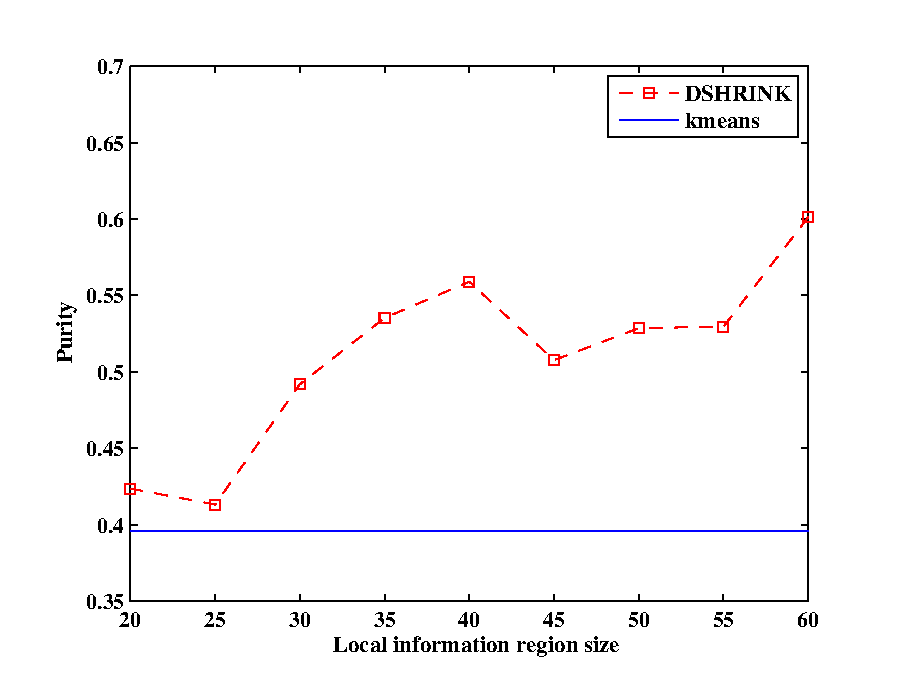
\includegraphics[width=0.45\textwidth]{blogcatalog_node_max.eps}}
  \subfigure[Blogcatalog-b]{
    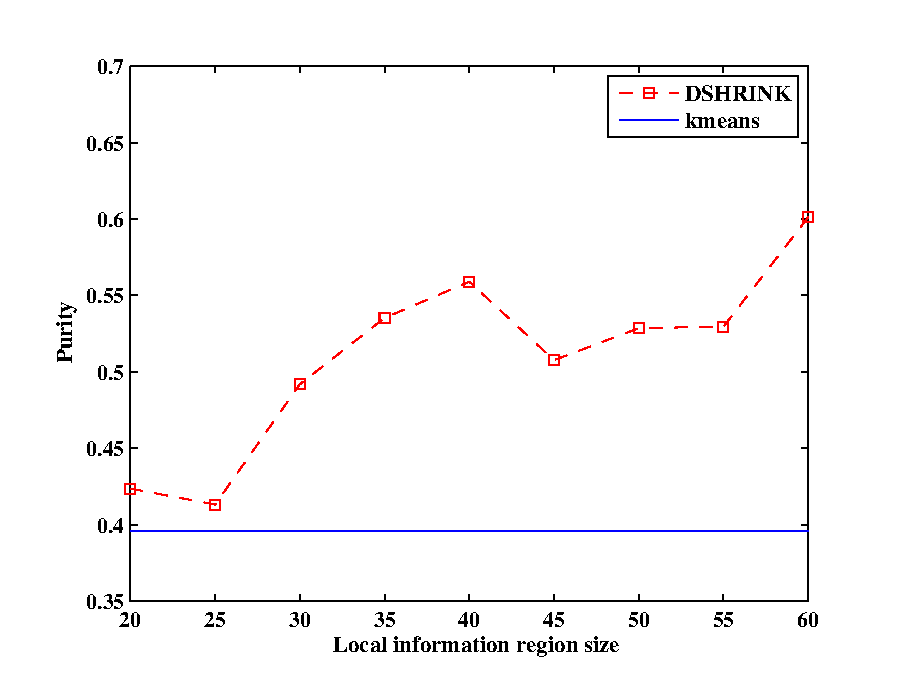
\includegraphics[width=0.45\textwidth]{blogcatalog_node_max.eps}}
\caption{不同局部信息网络大小下的纯度(局部信息网络个数为10)}
\end{figure}
\end{frame}

\begin{frame}{实验结果——不同局部信息网络个数}
\begin{figure}
  \centering
  \subfigure[Blogcatalog-a]{
    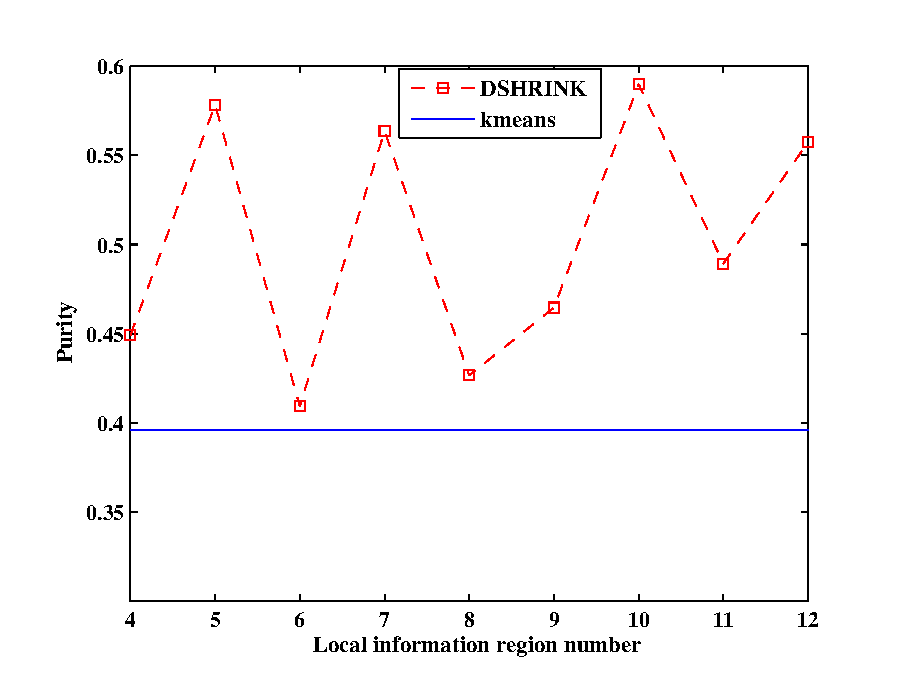
\includegraphics[width=0.45\textwidth]{blogcatalog_region_num.eps}}
  \subfigure[Blogcatalog-b]{
    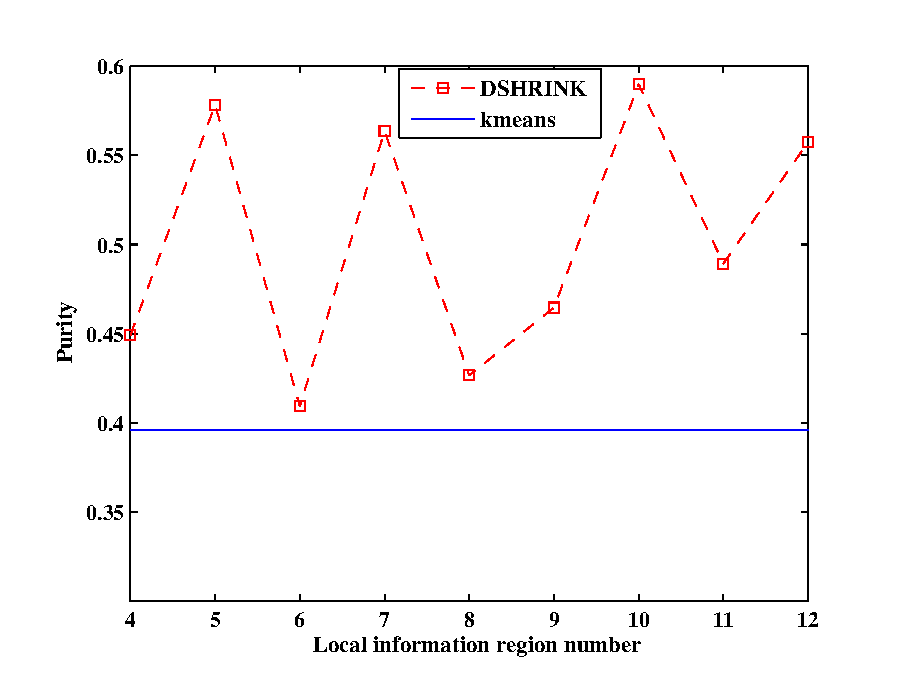
\includegraphics[width=0.45\textwidth]{blogcatalog_region_num.eps}}
\caption{不同局部信息网络个数下的纯度(局部信息网络大小为50)}
\end{figure}
\end{frame}


\begin{frame}{实验结果分析}
基于欧式距离进行调整 \pause

不需要先知道$k$
\end{frame}

%\section{枚举}

%\begin{frame}[fragile]{Ordered Lists}
%A Beamer theme consists of the following four parts: \pause
%\begin{enumerate}[<+->]
%\item outer theme, with \verb!\usebeameroutertheme!;
%\item inner theme, with \verb!\usebeamerinnertheme!;
%\item color theme, with \verb!\usebeamercolortheme!;
%\item font theme, with \verb!\usebeamerfonttheme!.
%\end{enumerate}
%\end{frame}

%\section{数学}

%\begin{frame}{Example}
%\begin{example}
%Prove the following result:
%\[ \lim_{x\to0}\frac{\sin 3x}{\ln(1-2x)}=-\frac{3}{2} \]
%\end{example}\pause
%\begin{proof}
%Since $\sin 3x \sim 3x$ and $\ln(1-2x) \sim -2x$, we have
%\[ \lim_{x\to0}\frac{\sin 3x}{\ln(1-2x)}=\lim_{x\to0}\frac{3x}{-2x}=-\frac{3}{2} \]
%\end{proof}
%\end{frame}

\section{致谢}

%\begin{frame}{致谢}
%\begin{center}
    %\bf{Thanks}
%\end{center}
%\end{frame}

\end{document}
